\documentclass[11pt,letterpaper]{article}

\newtheorem{theorem}{Theorem}
\newtheorem{corollary}{Corollary}
\newtheorem{lemma}{Lemma} 
\newtheorem{claim}{Claim}
\newtheorem{fact}{Fact}
\newtheorem{definition}{Definition}
\newtheorem{assumption}{Assumption}
\newtheorem{observation}{Observation}
\newtheorem{example}{Example}

\usepackage{epsfig}
\usepackage{graphicx}
\usepackage{amsmath}
\usepackage{amssymb}
\usepackage{enumerate}
\usepackage[margin=0.75in]{geometry}

\oddsidemargin 0in
\evensidemargin 0in
\textwidth 6.5in
\topmargin -0.5in
\textheight 9.0in
\abovecaptionskip 0in

\def\@maketitle
   {
   \newpage
   \null
   \vskip .375in
   \begin{center}
      {\Large \bf \@title \par}
      % additional two empty lines at the end of the title
      \vspace*{24pt}
      {
      \large
      \lineskip .5em
      \begin{tabular}[t]{c}
         \ifcvprfinal\@author\else Anonymous CVPR submission\\
         \vspace*{1pt}\\%This space will need to be here in the final copy, so don't squeeze it out for the review copy.
Paper ID \cvprPaperID \fi
      \end{tabular}
      \par
      }
      % additional small space at the end of the author name
      \vskip .5em
      % additional empty line at the end of the title block
      \vspace*{12pt}
   \end{center}
   }

\def\abstract
   {%
   \centerline{\large\bf Abstract}%
   \vspace*{12pt}%
   \it%
   }

\def\endabstract
   {
   % additional empty line at the end of the abstract
   \vspace*{12pt}
   }


\begin{document}
%%%%%%%%% TITLE
\title{CS224W Course Project Proposal: A survey of Network Alignment}

\author{Danqi Chen\\
Stanford University\\
{\tt\small danqi@stanford.edu}
% For a paper whose authors are all at the same institution,
% omit the following lines up until the closing ``}''.
% Additional authors and addresses can be added with ``\and'',
% just like the second author.
% To save space, use either the email address or home page, not both
\and
Botao Hu\\
Stanford University\\
{\tt\small botaohu@stanford.edu}
%
\and
Shuo Xie\\
Stanford University\\
{\tt\small shuoxie@stanford.edu}
}

\maketitle
\thispagestyle{empty}

\maketitle

%%%%%%%%% ABSTRACT
\begin{abstract}
   This document is a project proposal for the CS231A open course project. It details our plans for contributing to current research in real-time object tracking. Possible datasets, algorithms, readings  and evaluation methods are reviewed.
\end{abstract}

\section{Problem Statement}

\section{Algorithms}

\section{Data and Evaluation}

We will use the data from three large online social networks in our experiments: Twitter, Flickr and Foursquare. On these social networks, the data of user profiles and friendship connections are all public and accessable by crawlers or APIs. 

The first graph is the ``following'' relationships on the Twitter\footnote{http://www.twitter.com}, a microblogging service, which has 500 million users (200 million active). 

The second graph is the ``contact'' relationship on Flickr\footnote{http://www.flickr.com}, a photo-sharing service, which has 51 million registered members and 6 billion images on Jan 19, 2012.

The third graph is the ``Friends'' relationships on Foursquare\footnote{http://www.foursquare.com}, a location-based social network, which has 22 million global users on March 2, 2012. 



Narayanan at el. \ref{Narayanan2008} 

SNS 
Twitter
Flickr
Foursquare

Social structure data
Profile data

Foursquare 


\subsection{Ground truth}
To verify our de-anonymizing results , we have to determine the ground truth, i.e., the true mapping between the users of the online social networks. Actually, we do not need to label the mapping of all users since the ground truth as a test set can be far smaller than the complete network data.
Instead of labeling the user mapping by human editors, there are several sources to get the ground truth. 

\subsubsection{Single-source ground truth}

About.me\footnote{http://about.me} is a personal web hosting service, which had at least 1 million users on October, 2011 \footnote{http://techcrunch.com/2011/10/17/about-mes-ceo-on-how-to-hit-a-million-users-in-300-days-figure-out-who-your-entourage-is/}. The site offers registered users a simple platform from which to link multiple online identities, relevant external sites, and popular social networking websites such as Google+, Twitter, Facebook, LinkedIn, Flickr, YouTube, Foursquare. These links on user profile is naturally human-labelled mapping by the user itself, which can be seen as a zero-error ground truth.  We picked a random sample of the mappings and verified by human inspection that the most of about.me users have Twitter accounts and at least one of Flickr and Foursquare accounts. About.me also provides simple APIs to list user directory and view the links on user profile without the strict crawling limitation. Therefore, we will mainly adopt the data from about.me to be our ground truth in this project.

\subsubsection{Inferred multiple-source Ground truth}

The links of the user profile page of the social networking websites are another great sources for ground truth, which is also generated by the user itself. Usually, a single user has many accounts for different social networking website. On the user profile page, there might be links to this user's accounts in the other popular social networking webiste. Especially, nowadays, for the most the social networking website, the user logs in with the connection to his/her Twitter or Facebook account, and that website may show the user's Twitter and Facebook account in the user profile. For example, the figure \ref{fig:infer} shows how the links connects to other social networking website on the user profile page among the famous large social networking website: LinkedIn publicly shows the users' linked Twitter account and Gmail/Google+ account; and public Google+ profile reveals the user's Facebook and Twitter account; and Foursquare will show the user's login Twitter or Facebook account information. 

\begin{figure}[h!]
\centering
\caption{Links on the user profile page of serveral social networking website}
\label{fig:infer}
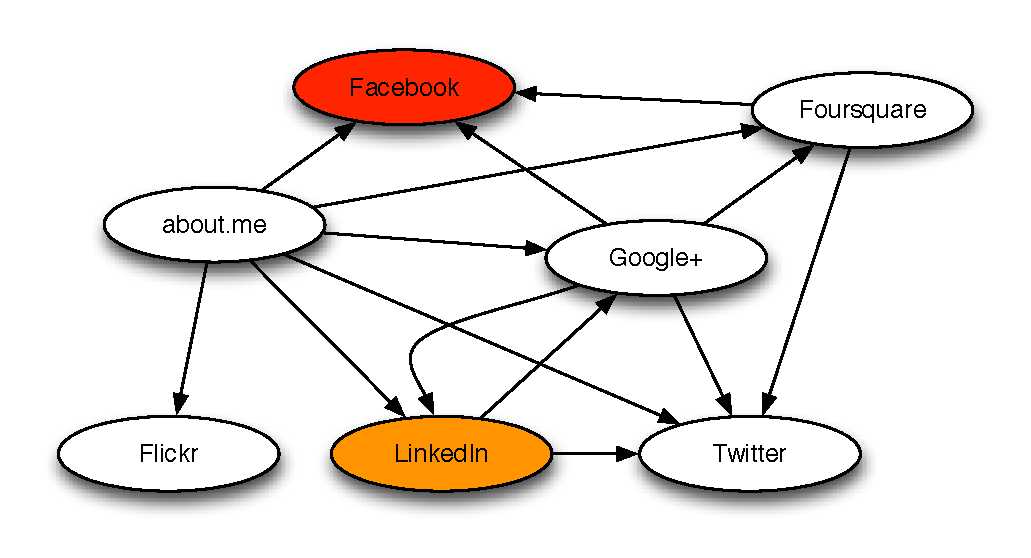
\includegraphics[width=0.7\textwidth]{infer.eps}
\end{figure}


Fortunately, on these famous social networking webiste in the figure \ref{fig:infer}, the most of user's profile pages are publicly accessbile. A crawler can easily follow these links on the profile page, discover all linked accounts about one user, and even retrieve the user's real name and affiliation from the profile on the real-name social networking website, such as LinkedIn and Facebook (colorred in orange and red in figure \ref{fig:infer}. Thus, we can build a ground truth by exploring all linked accounts of each user. 

\subsection{Evaluation}

Since we have a ground truth, correct matches 

We will compare Network Alignment \cite{Narayanan2008} and Simulated Annealling \cite{Kreitmann2011}. 

Belief Propagation

\section{Deliverable}
We hope to creata a final report, which 

We will implement the most of codes in SNAP\footnote{http://snap.stanford.edu} framework.  

\nocite{Ding2010,Wanga,Peng2012,Klau2009,Wondracek2010,Balduzzi2010,Koutra2011,Bayati2009,Bradde2010,Cromi2009,Flannick2009,Memisevic2012,Kreitmann2011,Narayanan2009,Delcher2002,Kollias2012,Mohammadi,Kuchaiev2007,Wangb,Liao2009,El-Kebir2011,Shi,Bayati2009a,Pache2012,Pache2012a,Kollias2011,Doan,Bayatia,Koyuturk2006,Todor2007,Narayanan2008,Burkhart2010,Backstrom2007}


\bibliographystyle{abbrv}
\bibliography{na}

\section{Appendix}

\end{document}
